\usetikzlibrary{patterns}

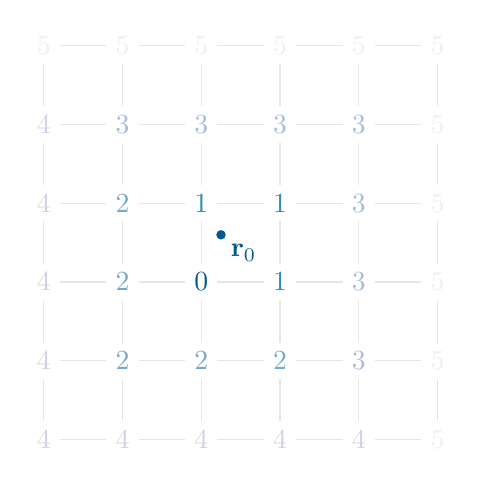
\begin{tikzpicture}
  \definecolor{cblue5}{HTML}{f1eef6}
  \definecolor{cblue4}{HTML}{d0d1e6}
  \definecolor{cblue3}{HTML}{a6bddb}
  \definecolor{cblue2}{HTML}{74a9cf}
  \definecolor{cblue1}{HTML}{2b8cbe}
  \definecolor{cblue0}{HTML}{045a8d}

  \draw[step=1.0,gray, opacity=0.2,thin] (-2,-2) grid (3,3);
  
  \draw[color=cblue0] (0,0) node[fill=white] {0};

  \fill[cblue0, radius=0.06] (0.25, 0.6) node[anchor=north west] {$\mathbf{r}_0$} circle;

  \foreach \i in {0, 1} {
    \draw[color=cblue1] (\i,1) node [fill=white] {1};
    \draw[color=cblue1] (1,\i) node [fill=white] {1};
  }

  \foreach \i in {-1, 0, 1} {
    \draw[color=cblue2] (\i,-1) node [fill=white] {2};
    \draw[color=cblue2] (-1,\i) node [fill=white] {2};
  }

  \foreach \i in {-1, 0, 1, 2} {
    \draw[color=cblue3] (\i,2) node [fill=white] {3};
    \draw[color=cblue3] (2,\i) node [fill=white] {3};
  }

  \foreach \i in {-2, -1, 0, 1, 2} {
    \draw[color=cblue4] (\i,-2) node [fill=white] {4};
    \draw[color=cblue4] (-2,\i) node [fill=white] {4};
  }

  \foreach \i in {-2, -1, 0, 1, 2, 3} {
    \draw[color=cblue5] (\i,3) node [fill=white] {5};
    \draw[color=cblue5] (3,\i) node [fill=white] {5};
  }
\end{tikzpicture}
